% Los objetivos específicos de cada uno de los subproyectos participantes, enumerándolos brevemente, con claridad, precisión y de manera realista (acorde con la duración prevista del proyecto).
%
% En los subproyectos con dos investigadores principales, deberá indicarse expresamente de qué objetivos específicos se hará responsable cada uno de ellos.
%

\subsubsection*{Objectives of the CALREC subproject}

The subproject CALREC, under the responsibility of the US, will provide the calibration systems for the NEW and NEXT-100 detectors (WP14).
In addition the US group will 
%develop tracking reconstruction algorithms for NEXT, will
take a leading role in the analysis of the NEW and NEXT-100 data  and will collaborate  in the R\& activities associated to \BATA. 

The specific objectives of this subproject are:
\begin{enumerate}
\item {\bf Design, construction, commissioning and operation of a calibration system to estimate the gain and noise of the SiPMs and PMTs sensors}. Two sets of 400 nm LEDs will be located on the tracking and energy planes. They will illuminate periodically the detector with a dim light. The gain and noise of SiPMs and PMTs will be estimated from single photo-electron signals. This procedure has been demonstrated in DEMO for the calibration of the energy plane. In NEW, we will apply it also to the calibration of the NEW SiPMs, which have much lower dark current than those deployed in DEMO and are, therefore, capable of counting single electrons.

\item {\bf Design, construction, commissioning and operation of an energy calibration system with external radioactive sources for NEW and NEXT-100}.
The energy scale and energy resolution in the region of \Qbb ~can be estimated using the photo-peak of the 2.6 MeV gamma from a \Tl~  source. In addition, the photo-peak electron and the two electrons of the double-scape peak (~1.6 MeV) can be used to measure the misidentification efficiency and the signal selection efficiency respectively. With additional 
\NA\ and \CS~ sources we can calibrate the energy scale in the range of 500 keV.

\item {\bf Design, construction, commissioning and operation of a position calibration system with X-rays}. X-rays from \Xe~ (30 keV) and \KR ~(42 keV) are point-like sources in NEXT.
They will be used to correct the bias on the energy introduced by geometrical effects and to estimate the light collection at the SiPMs from a point-like source (PSF function). This is a fundamental element for the tracking reconstruction algorithms. 

\item {\bf Design, implementation and validation of the tracking reconstruction algorithms of NEXT}.  The US co-coordinates the development of the NEXT reconstruction algorithms (the coordinator is the IP of this project and Dr. Ferrario, from IFIC) 


\item {\bf Take a leading role in analysis}. Design and do the measurement of the \bb~ spectrum with NEW data, and Design and prepare the search for \bbonu~  for NEXT-100. 
Again, calibration data from the radioactive sources will be crucial to estimate the efficiencies of the analysis.

\item {\bf Contribute to the \BATA\ R\&D}. In particular, US will lead the experiments focused in finding suitable additives for the xenon, such as TEA or TMA, capable to reduce transverse diffusion and increase drift velocity. The addition of additives may also be needed to transfer the charge from the Ba$^{++}$~ion produced in a \bb\ decay, to a Ba$^+$~ion which can be tagged with lasers.  
\end{enumerate}


\subsubsection*{Methodology of the CALREC project}

%4. El detalle de la metodología propuesta en cada uno de los subproyectos participantes, incluyendo la viabilidad metodológica de las tareas. Si fuera necesario, también se incluirá una evaluación crítica de las posibles dificultades de un objetivo específico y un plan de contingencia para resolverlas.
%

{\bf Calibration of SiPMs and PMTs sensors}

The gain and noise of the PMTs and SiPMs sensors will be calibrated with 400 nm LEDs located on the tracking and energy plane. 
Calibration data will be acquired during the physics runs.
%During the physics runs, the LEDs will illuminate the chamber at small rate.
The gain and noise will be obtained from a fit to the single photo-electron spectrum.
They will be monitored along time and temperature to correct for possible deviations. 
A similar method was already used to calibrate the PMTs of NEXT-DEMO\footcite{Lorca:2014sra}. No problems are expected here.

{\bf Energy calibration}

\begin{figure}
\begin{center}
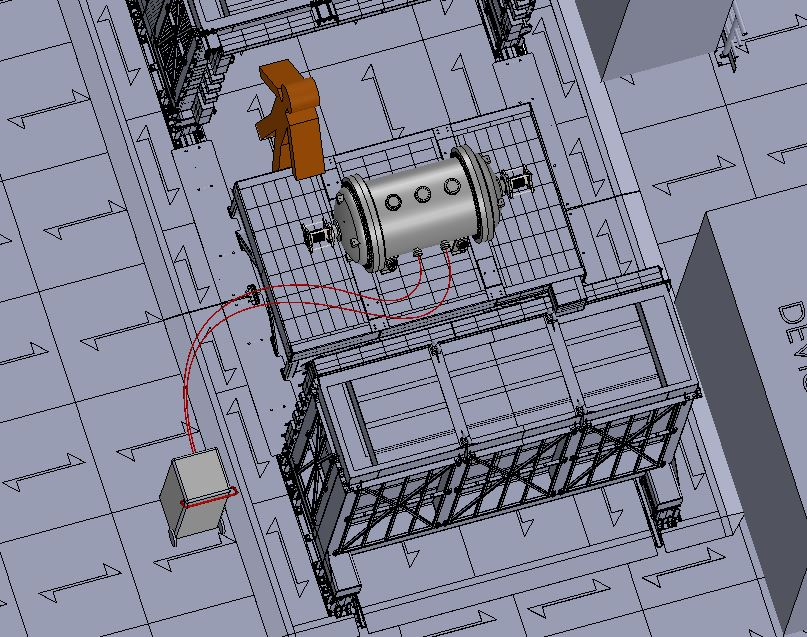
\includegraphics[width=0.6\textwidth]{src/CALREC/CALREC_LSC_sources.jpg}
%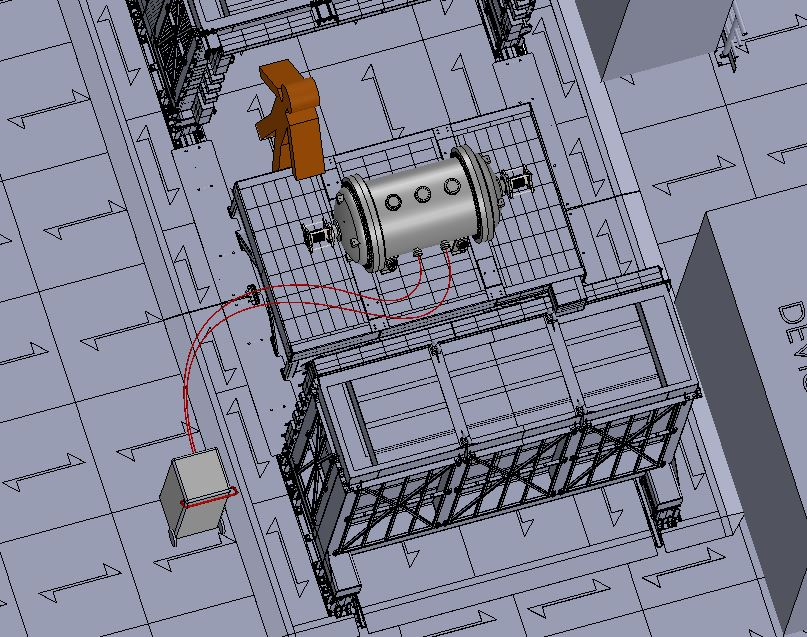
\includegraphics{img/CALIB_LSC_sources.jpg}
\caption{\small Drawing of the NEW detector at the LSC platform. The lead closet with the radioactive sources is on the left,  guides transmit gamas into the vessel via two ports on the side.}
\label{fig:CALREC_LSC_sources}
\end{center}
\end{figure}

To calibrate in energy, we will use several radiative sources.
\Tl ~emits a high energy gamma of 2.6 MeV and the double escape peak produces two electrons of $\sim$1.6 MeV energy.
The energy resolution and scale will be obtained from the width and position of the 2.6 MeV photo-peak, that is very close the \Qbb. 
From the two electrons at 1.6 MeV we can estimate the efficiency to identify a \bb\ signal.  
In addition to the \Tl, \NA ~(511 keV) and \CS ~(662 keV)  sources will be used to calibrate the energy scale around 500 keV. 

The sources will be located in a lead shielded closet outside the NEXT castle, a light guide will direct the gammas to the two ports on the side of the vessel  
(see Fig. \ref{fig:CALIB_LSC_sources}). 

Calibration runs will be taken periodically. Typically a long run per month should be enough, but the exact procedure will be defined as part of the commissioning process of NEW and then of NEXT-100.  

{\bf Calibration in Position}

Position calibration is needed to correct for the bias on the energy introduced by the geometry of the chamber. As demonstrated using NEXT-DEMO data\footcite{Lorca:2014sra} PMTs detect less light for events outside the central region of the detector. To correct for the geometrical dependence we will use X-rays from \Xe ~ (30 keV)  and \KR ~(42 keV). X-rays behave in the NEXT chambers as point like sources.
Corrections will be obtained from the measurement of the X-ray energy as a function of $z$ and the position on the transverse plane $x,y$.

A large statistic sample is necessary to map the full vessel volume.
For that reason, we plan to introduce \KR\ with the \Xe\ gas to increase the number of X ray interactions.  \KR\ has a half-life of $1.83 \pm 0.02$ hours and consequently 
it does not leave measurable traces trace in a few days. Also, being
a noble gas, it does not affect the purity of xenon.

The details of the calibration (injection, rates, etc) with \KR\ are still to be defined.
Most probably NEW will be calibrated with \KR\ on a monthly basis. The exact procedure will be defined as part of the commissioning process. 

%Notice also that X-rays could be used to estimate the Point Spread Function (PSF), the probability that light reach a given SiPM from a point-like source. We can study the PSF as a function of the position on the chamber. 
%This function a key ingredient for the reconstruction. 
%Algorithms to estimate the PSF from data need to be in place, but no difficulties are expected here.  
 
{\bf Reconstruction algorithms}

The reconstruction algorithms converts the calibrated signal from the SiPMs and PMTs into a 3D trajectory. Each point of the trajectory has associated a deposited energy. 
A trajectory is defined as single electron if one {\it blob} is found in one of the end-points of the trajectory and as a double electron if two blobs are found (see Figure \ref{fig.ETRK2}). 
A \bb\ signal candidate is always a double electron.  

During the DEMO phase of the project, we have developed a simple algorithms for electron reconstruction 
The simple one has been developed by the IFIC group for the NEXT-DEMO reconstruction \footcite{Alvarez:2012nd}. A collection of SiPMs are clustered together if they meet a given criteria of proximity and signal threshold. These clusters are connected into a 3D trajectory and an interpolation is done between the different points. This method is simple and good enough for an initial reconstruction but it lacks the capability to find complex structures as twists in the transverse plane, two segments in the same $z$ location or vertical tracks.
 
A second algorithm has been develop by the US group. It used the signal collected by the SiPMs and the Point Spread Function (PSF, the probability that light reach a given SiPM from a point-like source) to recover the image of the electron cloud at the EL using a Fast Fourier transform. The method is fast enough to process a large amount of data and provides the capability of finding complex structures in the transverse plane. 

Finally the third method, is being developed by the IFIC group under the coordination of Dr. Ferrario. The full detector volume is divided in $5\times5\times5$ mm$^3$ 3D boxes. Using the probability function that associates the deposited energy in a given 3D box with the signal detected at the SiPMs and PMTs, and via an iterative process, the method finds the 3D trajectory that maximises the likelihood that the detected signal match the image produced by the 3D trajectory. This is a time consuming algorithm but optimises energy resolution. Notice nevertheless, that it relies on the accurate estimation of the signal left on the PMTs and SiPMs from a deposition at a given point of the detector. 

NEW data will be essential to test, develop and further improve the above algorithms, optimising them to achieve the best posible energy resolution and track reconstruction during the physics run. Algorithms will be validated using simulated data, and real data from the \NA,  ~\CS ~and \Tl ~sources. 

{\bf \bb ~Analysis}

NEW will be able to measure the allowed \bb\ decay mode, \bbtnu. The measurement of the \bbtnu\ energy spectrum requires: a) definition of the signal region; b) estimation of the contamination events on that region; c) estimation of the signal yield, and d) a fine study of the measurement uncertainties.
Large MC samples will be used to define the signal selection. Multi-Variate Technique (such as Neural Network or Boosted Decision Trees) will be used to separate the signal from the background.
The efficiency of the selection and the contamination levels will be estimated from data, using the \Tl ~two-electrons from the doble scape peak at ~1.6 MeV and the photo-peak at 2.6 MeV, as discussed before. The expected background energy spectrum will be obtained from the radio purity measurements in conjunction with the detector simulation. Uncertainties on the spectrum around the region of interest will be carefully estimated.
The yield of \bb~ events will be obtained from the fit and used to measure the life-time of this process. 

The \bbonu\ search to be perform with NEXT-100 data is similar to the described above. The expected signal spectrum could be estimated from the famous \Tl ~2.6 MeV peak. 
Data will be fitted to all contributions, including a possible \bbonu ~signal.
From the estimated yield and detection efficiency, we could them measure, or set a limit in, the life-time on the \bbonu decay.

{\bf R+D with gas mixture}

Within this project the US will contribute to the R\&D of NEXT. Specifically, the responsibility of USC will be the study of additives (for example TMA, tre-methylamine) mixed with xenon.  These additives reduce the electron diffusion, which translate to a more confined trajectory.  In addition the scintillator light has  a 300 nm wavelength, easier to detect than the one of Xenon (170 nm). Last, but not least, some of the additives (including TMA) are capable of transferring the charge from the Ba$^{++}$~ion produced in a \bb\ xenon decay to
the Ba$^{+}$~ion which can be tagged (e.g., $Ba^{++} + A \rightarrow Ba^{+} + A^{+}$) where $A$~is the additive. US will coordinate a dedicated experiment to measure the kind of additive and the concentration needed for efficient charge transfer. 


\subsubsection*{CALREC subproject: Resources and equipment}

The CERN electronics laboratory at IFIC together with the work and test equipment at UPV (I3M institute and Gandia campus) provide enough resources for testing, debugging and prototyping electronics. High-performance signal analysers are available at IFIC, as well as specific instrumentation (from hand-held spectrum analysers to temperature meters) used in previous NEXT development stages.

\subsubsection*{CALREC subproject: schedule}
